\subsection{Eksisterende sociale robotter}
\label{EksisterendeSocialeRobotter}
%
Der findes et stort udvalg af sociale robotter når det kommer til børnelegetøj, blandt disse er den nok bedst kendte Sony's \textit{AIBO}, som er en robot hund, \parencite{WEB:AIBO}. \textit{AIBO} er designet til at udvikle sin personlighed fra hvalp til voksen, afhængigt af interaktionen med dens ejer og omgivelser, \parencite{WEB:AIBO}. \textit{AIBO} illustreres på \autoref{fig:EksisterendeSRAll}. Selvom \textit{AIBO} ikke er en virkelig hund, afspejler den hundes naturlige bevægelsesmønstre og behov, \parencite[ss. 191-198]{PDF:AnEthologicalEmotional}. Det resulterer i, at ejeren tildeler \textit{AIBO} hunde-agtige egenskaber, hvorved den behandles som en social ledsager med mentalkapacitet, \parencite[s. 2]{PDF:SharingALifeHarvey}. Dette kommer blandt andet til udtryk ved en analyse af kommentarer i et forum, hvor 47 \% tildeler \textit{AIBO} en biologisk essens, 42 \% vurderer at \textit{AIBO} har forsætlig adfærd, 38 \% vurderer at \textit{AIBO} har følelser og 39 \% vurderer at \textit{AIBO} kan opdrages, udvikles og modnes, \parencite[s. 26]{PDF:InTheCompanyofRobots}. En anden social robot, som ligeledes anvendes blandt børn er \textit{NAO}, designet af \textcite{WEB:NAO}. \textit{NAO} er en robot, der kan bruges til undervisning. \textit{NAO} illustreres på \autoref{fig:EksisterendeSRAll}.
%
\begin{figure}[H]
\centering
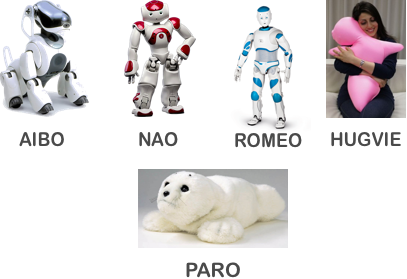
\includegraphics[width = 0.55\textwidth]{Figure/EksisterendeSRAll} 
\caption{Oversigt over et udvalg af eksisterende sociale robotter.}
\label{fig:EksisterendeSRAll}
\end{figure}
\noindent 
%  
I forbindelse med autistiske børn tyder det ligeledes på, at sociale robotter kan anvendes som en del af barnets terapi, \parencite[s. 180]{PDF:GamesChrildrenAutism}. Ifølge \textcite[s. 185]{PDF:GamesChrildrenAutism} er en af fordelene ved at anvende en robot, \textit{Roberta}, at den er mindre kompleks end mennesker, hvilket gør det muligt for robotten at hjælpe barnet med at udvikle sociale kompetencer.
  
Ydermere kan sociale robotter ligeledes indgå som en form for terapi for ældre, som eksempelvis lider at demens eller oplever ensomhed, \parencite[s. 110]{PDF:TheMobilePhoneAnEmontionalisedSR}. \textit{PARO}, som er en robot sæl, anvendes blandt andet i disse situationer. Ifølge \textcite{WEB:PARO}, reducerer \textit{PARO} patientens stress, gør dem mere afslappet og motiveret og forbedre socialeegenskaber. \textit{PARO} illustreres på \autoref{fig:EksisterendeSRAll}. Udover \textit{PARO}, findes \textit{ROMEO}, som er designet til at hjælpe ældre og andre der har mistet en del af deres mobilitet, \parencite{WEB:ROMEO}. \textit{ROMEO} illustreres på \autoref{fig:EksisterendeSRAll}. I forhold de før nævnte robotter er \textit{ROMEO} forholdvis stor; 140cm høj. Ved at introducerer sociale robotter, designet til at hjælpe ældre, kan det være med til at sænke belastningen på sundhedsystemet i takt med at den ældre har mulighed for et længere uafhængigt og sundere liv i sit eget hjem, \parencite[s. 1]{PDF:SharingALifeHarvey}.\blankline
% 
\textit{Double} tillader at medarbejdere kan arbejde hvor som helst og gennem robotten være til stede på arbejdspladsen samtidig, \parencite{WEB:Double}. \textit{Double} er illustreret på \autoref{fig:Double}. En lignende form for telekommunikation opleves med \textit{HUGVIE}, som er en menneskeformet pude med hovede, arme, krop og ben, \parencite[s. 78]{PDF:MinimizingTheHuman}. \textit{HUGVIE} illustreres på \autoref{fig:EksisterendeSRAll}. I \textit{HUGVIE}s hovede er det muligt at lægge en mobiltelefon i en lomme og dermed fører en samtale, eksempelvis med ens partner, samtidig med at brugeren krammer \textit{HUGVIE} og mærker dens hjertebanken, som afspejler den transmiterede lyd.

Derudover anvendes sociale robotter som turguider og receptionister på museer, \parencite[s. 22]{PDF:CloseButNotStuck}. Ved robotter såsom \textit{Rhino} og \textit{Minerva}, har fokus primært været på at udvikle navigation og undvigelsesmanøvre, \parencite[s. 318]{PDF:VisitingCulturalHeritage}. Ifølge \textcite[ss. 318-319]{PDF:VisitingCulturalHeritage} fokuserer tidligere undersøgelser, med forskellige sociale robotter brugt på museer, på et enkelt aspekt og ikke på evalueringen af hele brugeroplevelsen.     

